%%%%%%%% V2

\documentclass[12pt, a4paper]{article}

% =========================================================================
% PACKAGES & DOCUMENT GEOMETRY (100% OVERLEAF TEXLIVE COMPATIBLE)
% =========================================================================
\usepackage[utf8]{inputenc}
\usepackage[T1]{fontenc}
\usepackage{helvet}
\renewcommand{\familydefault}{\sfdefault}

\usepackage[margin=1.8cm, headheight=15pt]{geometry}
\usepackage{amsmath}
\usepackage{amssymb}
\usepackage{graphicx}
\usepackage{array}
\usepackage{tabularx}
\usepackage{booktabs}
\usepackage[table]{xcolor}
\usepackage{enumitem}
\usepackage{titlesec}
\usepackage{fancyhdr}
\usepackage{tocloft}
\usepackage{float}
\usepackage{tcolorbox}
\tcbuselibrary{breakable}
\usepackage{hyperref}
\usepackage{tikz}
\usetikzlibrary{positioning,arrows.meta,shapes.geometric}

% Automatically search both root folder and any images/ subfolder
\graphicspath{{./}{./images/}}

% =========================================================================
% FORMAL ACADEMIC COLOUR PALETTE (DELIVERABLE 1 STYLE)
% =========================================================================
\definecolor{AcademicNavy}{RGB}{20, 42, 74}
\definecolor{AcademicSlate}{RGB}{51, 65, 85}
\definecolor{BorderGray}{RGB}{203, 213, 225}
\definecolor{BgLight}{RGB}{248, 250, 252}
\definecolor{RowAlt}{RGB}{241, 245, 249}

\hypersetup{
    colorlinks=true,
    linkcolor=AcademicNavy,
    urlcolor=AcademicNavy,
    citecolor=AcademicNavy,
    linktoc=all
}

% =========================================================================
% SECTION & HEADER FORMATTING
% =========================================================================
\titleformat{\section}{\Large\bfseries\color{AcademicNavy}}{\thesection.}{0.5em}{}[\vspace{2pt}{\color{AcademicNavy}\titlerule[0.8pt]}]
\titleformat{\subsection}{\large\bfseries\color{AcademicSlate}}{\thesubsection}{0.5em}{}
\titlespacing*{\section}{0pt}{1.4em}{0.7em}
\titlespacing*{\subsection}{0pt}{1.0em}{0.4em}

\renewcommand{\cftsecleader}{\cftdotfill{\cftdotsep}}
\renewcommand{\cftsecfont}{\bfseries\color{AcademicNavy}}
\renewcommand{\cftsecpagefont}{\bfseries\color{AcademicNavy}}

\pagestyle{fancy}
\fancyhf{}
\fancyhead[L]{\small\textcolor{AcademicSlate}{COMP2300 Deliverable 2: Conceptual Design Report}}
\fancyhead[R]{\small\textcolor{AcademicSlate}{Arnav Mishra, Hiranya Makkar, Keshav Singhal}}
\fancyfoot[C]{\small\textcolor{AcademicSlate}{\thepage}}
\renewcommand{\headrulewidth}{0.4pt}

\setlength{\parindent}{0pt}
\setlength{\parskip}{0.55em}
\setlist[itemize]{leftmargin=1.5em, itemsep=0.25em, topsep=0.2em}

% =========================================================================
% SAFE IMAGE RENDERER (AUTOMATICALLY RENDERS pic1.png - pic9.png)
% =========================================================================
\newcommand{\renderpic}[3]{%
    \IfFileExists{#1}{%
        \includegraphics[width=#2, height=#3, keepaspectratio]{#1}%
    }{%
        \fbox{\parbox[c][0.22\textheight][c]{#2}{\centering\small\textbf{Image Ready: \texttt{#1}}\\[4pt]Upload \texttt{#1} to your Overleaf project root to display automatically.}}%
    }%
}

% =========================================================================
% ACADEMIC SPECIFICATION BOX FOR USER STORIES
% =========================================================================
\newtcolorbox{storybox}[2]{
    breakable,
    colback=BgLight,
    colframe=AcademicNavy,
    colbacktitle=AcademicNavy,
    coltitle=white,
    fonttitle=\bfseries\normalsize,
    title={#1 \hfill {\small\normalfont\textcolor{white}{#2}}},
    boxrule=0.7pt,
    arc=2pt,
    left=8pt,
    right=8pt,
    top=6pt,
    bottom=6pt,
    before skip=8pt,
    after skip=8pt
}

\begin{document}

% =========================================================================
% TITLE PAGE BLOCK
% =========================================================================
\begin{center}
    \vspace*{0.5em}
    {\LARGE\bfseries\color{AcademicNavy} Footprint Lens: Contextual Choice Coach}\\[0.5em]
    {\Large\bfseries COMP2300 Deliverable 2: Conceptual Design Report}\\[0.3em]
    {\normalsize\itshape\color{AcademicSlate} Topic 1: Carbon Footprint Awareness and Reduction Tool (Urban India Context)}\\[1.2em]

    \begin{tabular}{ll}
        \textbf{Module:}  & COMP2300 Software Design and Development Project \\
        \textbf{Date:}    & November 2026 \\
        \textbf{Version:} & 2.1 (Revised Conceptual Design Draft) \\
        \textbf{Authors:} & Arnav Mishra (\texttt{am31g25@soton.ac.uk}) \\
                          & Hiranya Makkar (\texttt{hm8g25@soton.ac.uk}) \\
                          & Keshav Singhal (\texttt{ks3e25@soton.ac.uk})
    \end{tabular}
\end{center}
\vspace{0.8em}

% =========================================================================
% TABLE OF CONTENTS (INDEX)
% =========================================================================
{\color{AcademicNavy}\hrule height 0.8pt}
\vspace{0.3em}
\tableofcontents
\vspace{0.5em}
{\color{AcademicNavy}\hrule height 0.8pt}
\newpage

% =========================================================================
% SECTION 1: PROBLEM SPACE ALIGNMENT
% =========================================================================
\section{Problem Space Alignment and Deliverable 1 Traceability}
This conceptual design directly operationalises the 62-word Job to Be Done (JTBD) established in Deliverable 1, maintaining strict traceability to our thematic analysis of interview transcripts \texttt{CF1}--\texttt{CF10}:

\begin{tcolorbox}[colback=BgLight, colframe=AcademicNavy, boxrule=0.7pt, arc=2pt, left=10pt, right=10pt, top=6pt, bottom=6pt]
\textit{``When I want to understand how my everyday routines and household habits affect the environment, I want to see which activities matter most in terms I can picture and which realistic alternatives are open to me, so that I can make changes that fit my budget, safety, rota, and shared home without being misled, lectured, or blamed for constraints I cannot control.''}
\end{tcolorbox}

To ensure full continuity between problem definition and conceptual architecture, our design maps to all six Deliverable 1 personas across three primary stakeholder groups and four operational scenarios:
\begin{itemize}
    \item \textbf{Urban Students and Shared-Housing Youth:} \textbf{P1 Ananya Deshmukh} (Age 21, Pune engineering hostel student navigating 10:30 PM gate curfews, 3 AM exam deliveries, shared floor geysers, and limited mobile data) and \textbf{P2 Karthik Sundaram} (Age 24, Chennai Environmental Science postgraduate requiring transparent Indian coal-grid factors, electronics repair logging, and CSV export alongside a simple view for co-living flatmates).
    \item \textbf{Time-Poor Urban Working Professionals:} \textbf{P3 Rohan Kulkarni} (Age 29, hybrid software engineer and composite persona relocated to the Chennai 2BHK co-living scenario in D1, seeking practical WFH AC comparisons and phone-longevity prompts) and \textbf{P4 Priya Reddy} (Age 31, Hyderabad rotating night-shift nurse requiring safety-locked night cab exemptions and muted daytime sleep windows).
    \item \textbf{Multi-Generational Household Managers and Elders:} \textbf{P5 Sunita Sharma} (Age 46, Noida 3BHK homemaker managing LPG pressure cooking, terrace composting, \textit{kabadiwala} recycling, and teen shower conflicts) and \textbf{P6 Rajeshwar Prasad Verma} (Age 58, retired railway official originally represented by CF8 in Lucknow and relocated in D1’s composite SC1 household to live with Sunita in Noida; he needs Plain Hindi, bucket-water metrics, and hourly fan costs).
    \item \textbf{Core Structural Scenarios:} \textbf{SC1} (Noida 3BHK multi-generational utility and water-bucket conflict), \textbf{SC2} (Pune hostel exam-week quick-commerce and shared geyser disaggregation), \textbf{SC3} (Hyderabad night-shift rota scheduling and safety-cab protection), and \textbf{SC4} (shared co-living bill audit, WFH AC, and phone longevity in a Chennai 2BHK).
\end{itemize}


\subsection{Research Basis for the Design Constraints}
The India-specific framing is consistent with research showing that household carbon footprints vary across household, city, and regional contexts; this supports avoiding a single undifferentiated global profile for all users \cite{lee2021}. More broadly, carbon-footprint research spans multiple methods and scales, so the provenance and system boundary of each factor must remain inspectable rather than being hidden behind a single score \cite{shi2021}.

The decision to use contextual feedback without coercive rankings is also grounded in prior work. Research on sustainability interfaces cautions that persuasive framings can narrow users' understanding of sustainability and overlook the situated nature of everyday practices \cite{brynjarsdottir2012}. Studies of carbon-footprint tracking applications examine engagement and behavioural outcomes, supporting the need to evaluate how feedback is interpreted rather than assuming that displaying a footprint automatically changes behaviour \cite{hoffmann2024,lasarov2024}. Work on quantified environmental feedback further motivates testing whether familiar comparisons improve comprehension, while avoiding the implication that unlike measures are interchangeable \cite{mohanty2023}.

These publications inform the design rationale; they do not validate the Footprint Lens prototype. The proposed interaction choices remain hypotheses to be examined through the formative evaluation in Section 6.

% =========================================================================
% SECTION 2: DESIGN CONCEPT GENERATION
% =========================================================================
\section{Design Concept Generation}

\subsection{Ideation Process and Evidence}
The three alternatives in this report are a retrospective synthesis of the problem constraints established in Deliverable 1, rather than a claim that a fully documented, time-stamped ideation workshop was conducted. The alternatives deliberately represent different interaction paradigms: automated retrospective capture, communal visibility, and personal decision support. This distinction allowed the team to compare different assumptions about data collection, user agency, privacy, and the timing of feedback.

The concepts were examined against the D1 personas, scenarios, semantic and latent themes, and research questions. The comparison below records the design space considered and the principal trade-off associated with each direction. No workshop date, participant count, idea count, or named ideation technique is claimed because those details are not evidenced in the current project record. Original sketches or meeting notes retained by the team may be added as supplementary process evidence; they are not represented here as contemporaneous artefacts.

\begin{table}[H]
\centering
\small
\renewcommand{\arraystretch}{1.3}
\begin{tabularx}{\textwidth}{@{}p{2.7cm} X X@{}}
\toprule
\textbf{Interaction paradigm} & \textbf{Core interaction model} & \textbf{Principal design trade-off} \\
\midrule
A: Passive Ledger & Retrospective import of utility bills, transaction exports, and device data to generate an aggregated audit. & Low routine-entry effort, but greater privacy, integration, and accessibility costs; limited point-of-decision guidance. \\
B: Social Kiosk & Shared household or hostel display for communal resource use and group-level feedback. & Makes shared consumption visible, but creates risks of unwanted attribution, social comparison, and household policing. \\
C: Hybrid Simulator & Manual low-friction logging with contextual feedback, inspectable assumptions, and optional decision-support branches. & Requires some user input, but offers greater transparency, user agency, and feasibility within the proposed offline-first scope. \\
\bottomrule
\end{tabularx}
\caption{Retrospective synthesis of the three interaction paradigms considered in D2.}
\label{tab:concept-paradigms}
\end{table}

In accordance with the COMP2300 Deliverable 2 specification, the alternatives represent distinct interaction models rather than minor visual variations. Each was considered against the D1 semantic themes (S1--S3), latent themes (L1--L3), and research questions (RQ1--RQ3).


\subsection{Concept A: Passive Ledger (Automated Receipt and Smart-Plug Auditor)}
Concept A operates as a background desktop financial and utility ledger. Rather than prompting users for daily habit check-ins, the proposed system ingests monthly state electricity board PDFs, exported Swiggy, Zomato, and Amazon order history CSVs, and automated smart-plug wattage logs to compile a retrospective end-of-month carbon and Rupee audit.
\begin{itemize}
    \item \textbf{Operational Mechanics:} Users drag-and-drop monthly billing statements into a parser table. The proposed system applies top-down Input-Output Analysis (IOA) spend multipliers to categorise food delivery packaging, apparel purchases, and appliance kWh usage, producing a monthly financial-environmental balance sheet tailored to \textbf{P3 Rohan} (\texttt{CF2}) and \textbf{P2 Karthik} (\texttt{CF4}).
    \item \textbf{Critical Limitations and Rejection Rationale:} While Concept A reduces daily typing for tech-savvy professionals, it fails our core accessibility and scope criteria. First, it alienates \textbf{P1 Ananya} (\texttt{CF1}) and \textbf{P6 Rajeshwar} (\texttt{CF8}), who do not export e-commerce CSV files or own smart-home telemetry hardware. Second, automated bank and order scraping violates Epic \textbf{E14} (\textit{Won't Have: external account scraping and cloud dependencies in v1.0}). Third, retrospective end-of-month audits provide zero point-of-decision guidance when a user is deciding whether to reduce WFH air-conditioning use (\textbf{SC4}).
\end{itemize}

\subsection{Concept B: Social Kiosk (Communal Household and Hostel Challenge Board)}
Concept B reframes carbon tracking as a shared, ambient household kiosk designed for a family tablet or co-living common-room monitor. It focuses exclusively on collective resource consumption, converting shared electricity bills and municipal water-tanker deliveries into room-by-room splits and competitive household leaderboards.
\begin{itemize}
    \item \textbf{Operational Mechanics:} Household members log shower durations, geyser timer activations, and AC hours onto a central floor board. The interface visualises communal totals in 15-litre water buckets and Rupees, ranking flatmates or family members on a weekly efficiency leaderboard to address \textbf{P5 Sunita}'s (\texttt{CF3}) frustration with unmonitored teen showers in \textbf{SC1}.
    \item \textbf{Critical Limitations and Rejection Rationale:} Despite addressing shared water and energy visibility (\textbf{L2}), Concept B introduces severe socio-technical risks. Publicly ranking individuals on a communal board violates Epic \textbf{E13} (\textit{Won't Have: forced roommate bill-splitting and public shaming leaderboards}) and fails \textbf{RQ3}. In shared student hostels (\textbf{SC2}) or co-living flats (\texttt{CF10}), exposing individual usage without voluntary consent triggers interpersonal conflict. Furthermore, Concept B provides no support for solo rotating shift workers like \textbf{P4 Priya} (\textbf{SC3}) and lacks the granular formula provenance required by \textbf{P2 Karthik} (\textbf{E2}).
\end{itemize}

\subsection{Concept C: Hybrid Simulator (Dual-Mode Adaptive Companion --- Selected)}
Concept C synthesises low-friction daily logging with an interactive decision sandbox inside an offline-first desktop application. It pairs a \textbf{Simple Companion View} (driven by 2-tap presets and Plain Hindi/vernacular toggles) with an on-demand \textbf{Detailed Researcher Audit View} (providing inspectable emission factors and, in a later increment, local CSV export).
\begin{itemize}
    \item \textbf{Operational Mechanics:} Users define their session scope and safety/shift constraints at entry (\textbf{State P0}), log routines in under 60 seconds using 2-tap preset cards or single-field quantities (\textbf{State P1}), and immediately inspect their impact paired with Rupees, 15L water buckets, and city bus trips alongside a live ``What-If'' habit swap slider (\textbf{State P2}). Domain experts can open the Provenance Inspector (\textbf{State P3}) to edit the Central Electricity Authority (CEA) grid factor ($0.716\text{ kg CO}_2\text{/kWh}$ (provisional D1 assumption; source and year require verification)) or local tariff ($\text{Rs. }8.00\text{/kWh}$). Crucially, Concept C enforces a \textbf{Constraint Shield} (\textbf{State P4}) that exempts night-shift safety cabs and daytime sleep AC from moralising penalties (\textbf{L3}), records traditional repair and composting habits descriptively without fabricating fake carbon offsets (\textbf{State P5}), and defaults shared household bills to communal totals with strictly voluntary opt-in attribution (\textbf{State P6}).
    \item \textbf{Selection Justification:} Concept C is the strongest of the three alternatives against the four D1 scenarios (\textbf{SC1}--\textbf{SC4}) and provides a plausible design response for all six personas (\textbf{P1}--\textbf{P6}) through progressive disclosure; this fit remains to be evaluated with users. It is designed to address \textbf{RQ1} (tangible unit comprehension), \textbf{RQ2} (2-tap low-friction logging), and \textbf{RQ3} (non-policing household boundaries) while remaining feasible as a bounded Java/JavaFX desktop MVP with local persistence, subject to implementation and testing in later deliverables.
\end{itemize}

% =========================================================================
% SECTION 3: CONCEPT SELECTION ANALYSIS (MCDM)
% =========================================================================
\section{Concept Selection Analysis (MCDM)}
Table \ref{tab:mcdm} presents the Multi-Criteria Decision Analysis (MCDM) used to evaluate the three concepts against weighted engineering and human-factors criteria derived from Deliverable 1.

\begin{table}[H]
\centering
\small
\renewcommand{\arraystretch}{1.45}
\begin{tabularx}{\textwidth}{@{} >{\bfseries}p{3.0cm} c X X X @{}}
\toprule
\rowcolor{AcademicNavy}
\textcolor{white}{Criterion} & \textcolor{white}{Weight} & \textcolor{white}{Concept A: Passive Ledger} & \textcolor{white}{Concept B: Social Kiosk} & \textcolor{white}{Concept C: Hybrid Simulator} \\
\midrule
D1 Must Epics (E1--E5) & 25\% & \textbf{2.0 / 5.0}\newline Fails E3 safety shields and E5 2-tap manual entry. & \textbf{3.0 / 5.0}\newline Supports buckets (E1) but weak on E2 formula audit and E3. & \textbf{4.5 / 5.0}\newline Provides conceptual coverage of E1--E5 through manual entry, inspectable assumptions, protected-routine handling, descriptive records, and offline operation; some requirements still need evaluation. \\
\rowcolor{RowAlt}
Persona \& Scenario Fit & 25\% & \textbf{2.5 / 5.0}\newline Excludes P1 (student) and P6 (elder) who lack CSVs. & \textbf{3.5 / 5.0}\newline Fits SC1 families but fails solo shift nurse P4 (SC3). & \textbf{4.5 / 5.0}\newline Serves P1--P6 across SC1--SC4 via dual-mode views. \\
JavaFX Offline Feasibility & 20\% & \textbf{2.5 / 5.0}\newline Bill/PDF parsing is brittle and risks E14 scope creep. & \textbf{2.5 / 5.0}\newline Multi-device sync adds unnecessary network overhead. & \textbf{4.5 / 5.0}\newline A bounded JavaFX/MVVM design with local JSON persistence appears feasible; implementation and integration risks remain. \\
\rowcolor{RowAlt}
Transparency \& Provenance & 15\% & \textbf{3.0 / 5.0}\newline Spend multipliers act as an opaque black box. & \textbf{3.0 / 5.0}\newline Prioritises gamified badges over visible assumptions. & \textbf{4.0 / 5.0}\newline State P3 exposes assumptions and provenance, but the factor source/year still requires verification. \\
Socio-Technical Risk Profile & 15\% & \textbf{3.0 / 5.0}\newline High privacy concern around financial statement import. & \textbf{2.0 / 5.0}\newline High risk of roommate policing friction (violates E13). & \textbf{4.5 / 5.0}\newline Voluntary opt-in (P6) and no fake offsets (P5) minimise risk. \\
\midrule
\textbf{Weighted Total} & \textbf{100\%} & \textbf{2.53 / 5.00} & \textbf{2.88 / 5.00} & \textbf{4.43 / 5.00 (Selected)} \\
\bottomrule
\end{tabularx}

\caption{Multi-Criteria Decision Matrix justifying the selection of Concept C.}


\label{tab:mcdm}
\end{table}

\textbf{Scoring method and anchors.} Each criterion is rated on a five-point ordinal scale. A score of \textbf{1} indicates conflict with the criterion or negligible coverage; \textbf{2} indicates substantial gaps; \textbf{3} indicates partial coverage with material limitations; \textbf{4} indicates good coverage with manageable limitations; and \textbf{5} indicates strong alignment with no major conceptual conflict identified. For feasibility, a 5 means the proposed scope can reasonably be represented within the target JavaFX/offline architecture, not that implementation has already been proven. For persona and scenario fit, a 5 requires a credible response across mapped D1 personas and scenarios, rather than merely mentioning them.

The weighted total is calculated as $\sum_i w_i s_i$, where the weights sum to 1. The totals are A = 2.53, B = 2.88, and C = 4.43 (rounded to two decimal places). These values are structured team judgements based on the design rationale in this report; they are not measured user outcomes. Concept C's high ratings express its relative alignment with the stated constraints and bounded scope. They remain hypotheses to be challenged through formative evaluation, particularly for multilingual comprehension, low-friction entry, and household consent boundaries.

\newpage

% =========================================================================
% SECTION 4: DETAILED USER STORY REGISTER (FULL-SPACE CARDS)
% =========================================================================

\subsection{D1 Priority and Scope Baseline}
The story register preserves the priority decisions in D1 Section 4. The D2 prototype may visualise Should-Have and Could-Have ideas to make the concept discussable, but this does not promote them into the v1.0 Must-Have implementation scope.

\begin{table}[H]
\centering
\small
\begin{tabularx}{\textwidth}{@{}l l X@{}}
\toprule
\textbf{D1 priority} & \textbf{Epics} & \textbf{D2 treatment} \\
\midrule
Must Have & E1--E5 & Core conceptual journey: estimate, assumptions, constraint protection, circularity record, low-effort offline entry. \\
Should Have & E6--E9 & Optional comparison, shared-household view, review summary, and detailed audit/export (CSV in Increment 2). \\
Could Have & E10--E12 & Rota timing, static reference-flat benchmarks, and smart-plug timer helpers; future increments only. \\
Won't Have & E13--E14 & No public rankings, forced attribution, automated account/hardware scraping, or unverified offset credits in v1.0. \\
\bottomrule
\end{tabularx}
\caption{D1 MoSCoW priorities carried forward into D2.}
\label{tab:priority-trace}
\end{table}

\section{Detailed User Story Register (Epics E1--E14)}
Concept C is decomposed into user stories mapped to the fourteen D1 epics (\textbf{E1}--\textbf{E14}). The D1 MoSCoW priorities remain authoritative: E1--E5 Must, E6--E9 Should, E10--E12 Could, and E13--E14 Won't Have. Each specification defines the MoSCoW priority, target personas, scenario links, and testable Behavior-Driven Development (BDD) acceptance criteria (\textit{Given / When / Then}) to govern Deliverable 3 evaluation and Deliverables 4--6 JUnit verification.

\begin{storybox}{US01 (Epic E1): Tangible Dual-Unit Metric Translation}{MoSCoW: Must Have | Personas: P1, P3, P5, P6 | Scenarios: SC1--SC4}
\textbf{User Story:} As an urban Indian user unfamiliar with abstract climate metrics, I want an estimate accompanied by relevant, clearly labelled everyday measures where defensible (Indian Rupees, 15-litre water buckets, fan/AC hours, and city bus trips) alongside $\text{kg CO}_2$, so that I can immediately picture the real-world scale of my household and commuting routines.
\begin{itemize}
    \item \textbf{Given} a valid routine quantity is entered or selected via preset in State P1 (e.g., $168.0\text{ kWh}$ monthly electricity),
    \item \textbf{When} the calculation engine executes the emission conversion strategy,
    \item \textbf{Then} State P2 displays the illustrative electricity result ($120.29\text{ kg CO}_2$) beside the assumed electricity cost (Rs. 1,344). The interface labels the factor as provisional and does not imply that water volume or currency is a carbon equivalent.
\end{itemize}
\end{storybox}

\begin{storybox}{US02 (Epic E2): Transparent Assumption Inspection and Live Editing}{MoSCoW: Must Have | Personas: P2, P3, P5, P6 | Scenarios: SC1--SC4}
\textbf{User Story:} As an evidence-conscious researcher or analytical householder, I want to inspect and edit the underlying conversion assumptions (regional CEA coal-grid factor, electricity tariff rate, and mathematical formula), so that I can verify where estimates come from and calibrate them to my state electricity board bill.
\begin{itemize}
    \item \textbf{Given} a calculated routine footprint in State P2,
    \item \textbf{When} the user opens the assumptions panel and changes an editable illustrative parameter (for example, the grid factor or tariff),
    \item \textbf{Then} the interface displays the revised formula and recalculated estimate, while retaining the parameter's unit, source, geography, reference year, and provisional status.
\end{itemize}
\end{storybox}

\begin{storybox}{US03 (Epic E3): Structural Constraint Shield for Safety and Shift Routines}{MoSCoW: Must Have | Personas: P1, P3, P4 | Scenarios: SC2--SC4}
\textbf{User Story:} As a user whose routine is constrained by safety, health, housing, or work conditions, I want to flag non-negotiable activities (such as a night-shift safety cab, essential cooling during daytime sleep, or a hostel curfew constraint), so that the tool does not frame an infeasible change as a personal failure.
\begin{itemize}
    \item \textbf{Given} the user checks the \textit{Protected Health/Safety Routine} checkbox in State P0,
    \item \textbf{When} the user views the Constraint Shield action screen in State P4,
    \item \textbf{Then} the protected routine is visibly labelled \textit{Protected}; no reduction prompt, negative score, or penalty is displayed for it. Optional actions remain available only for routines not marked as protected.
\end{itemize}
\end{storybox}

\begin{storybox}{US04 (Epic E4): Descriptive Circularity and Low-Waste Habit Recognition}{MoSCoW: Must Have | Personas: P1--P6 | Scenarios: SC1--SC4}
\textbf{User Story:} As a user practising lower-waste and circular activities, I want relevant actions (including repair and longer product use, composting, recycling, food-waste reduction, reusable packaging, and lower-waste food or clothing choices) recorded honestly, so that the tool recognises these practices without inventing unsupported carbon savings.
\begin{itemize}
    \item \textbf{Given} the user selects a supported circularity or lower-waste category (for example, repair, composting, recycling, food-waste reduction, or reusable packaging) in State P5,
    \item \textbf{When} the habit is saved with the optional descriptive-summary setting selected,
    \item \textbf{Then} the system logs the practice as a descriptive record (not a verified environmental-impact claim) explicitly labelled \textit{Status: Estimate Unavailable (No Fake Offsets)} and never subtracts fabricated $\text{kg CO}_2$ deductions from direct energy totals.
\end{itemize}
\end{storybox}

\begin{storybox}{US05 (Epic E5): Offline 2-Tap Preset Logger and Plain Hindi Toggle}{MoSCoW: Must Have | Personas: P1, P2, P4, P5, P6 | Scenarios: SC1--SC4}
\textbf{User Story:} As a time-poor user who may have limited connectivity or prefer a familiar language, I want routine presets and an English / Plain Hindi interface that remains usable offline, with relevant local-language guidance cards for the contexts identified in D1, so that I can record a routine with minimal effort.
\begin{itemize}
    \item \textbf{Given} the application is running with zero network connectivity,
    \item \textbf{When} the user has completed initial language and scope setup and selects one preset in State P1,
    \item \textbf{Then} the selected preset fills its quantity and unit and can be submitted without a network connection. The design target is no more than two logging actions and 60 seconds for a familiar preset task; both measures are evaluated rather than assumed. English and Plain Hindi are the initial interface options; additional language cards identified in D1 for SC2 and SC4 are content extensions, not a claim of complete interface localisation.
\end{itemize}
\end{storybox}

\begin{storybox}{US06 (Epic E6): Side-by-Side What-If Habit Swap Simulator}{MoSCoW: Should Have | Personas: P1, P3, P5 | Scenarios: SC1, SC3, SC4}
\textbf{User Story:} As a decision-maker comparing everyday alternatives, I want an interactive What-If slider that previews the estimated changes in Rupee cost and emissions of a realistic adjustment (such as cutting WFH AC runtime by 1 hour or swapping one car commute to the Metro), so that I can evaluate trade-offs before committing.
\begin{itemize}
    \item \textbf{Given} a baseline routine calculation in State P2 ($168.0\text{ kWh} = 120.29\text{ kg CO}_2$ using the provisional D1 assumption),
    \item \textbf{When} the user adjusts the \textit{What-If Swap Simulator} slider (\textit{Cut 1.5 kW WFH AC 1 hr early}),
    \item \textbf{Then} the simulator displays the estimated difference beside the baseline and exposes the assumptions used. Under the D1 illustrative assumptions (1.5 kW, one hour, 14 days, 0.716 kg CO$_2$/kWh, Rs. 8/kWh), the example is 21 kWh, approximately 15.04 kg CO$_2$, and Rs. 168; these are scenario outputs, not guaranteed savings.
\end{itemize}
\end{storybox}

\begin{storybox}{US07 (Epic E7): Shared Household Boundary with Voluntary Opt-In}{MoSCoW: Should Have | Personas: P1, P2, P3, P5, P6 | Scenarios: SC1, SC2}
\textbf{User Story:} As a resident in a multi-generational home or shared student flat, I want shared utility bills displayed as a communal total by default with a strictly voluntary opt-in toggle for my own room share, so that we can coordinate household reductions without policing or blaming flatmates.
\begin{itemize}
    \item \textbf{Given} \textit{Household Scope} is selected for a shared bill ($168\text{ kWh}$) in State P6,
    \item \textbf{When} the Shared Household Boundary view loads,
    \item \textbf{Then} it displays the \textit{Communal Total (Default)} and the rule \textit{``Shared bills do not equal personal footprints''}; only the active user can opt in to displaying their own share, and no other resident's usage is inferred or exposed without consent.
\end{itemize}
\end{storybox}

\begin{storybox}{US08 (Epic E8): Non-Judgmental Monthly Summary and Single Challenge}{MoSCoW: Should Have | Personas: P1, P3, P5 | Scenarios: SC3, SC4}
\textbf{User Story:} As a user fatigued by moralising eco-guilt, I want a clean monthly category breakdown paired with a single optional monthly challenge (such as keeping a smartphone an extra year or batching grocery orders), so that I can track progress without punitive streak counters.
\begin{itemize}
    \item \textbf{Given} the user has logged one or more routines during the selected calendar month,
    \item \textbf{When} the monthly summary is viewed,
    \item \textbf{Then} the summary shows the selected month, groups available records by domain (Energy, Mobility, Delivery/Packaging, Circularity), and distinguishes unavailable estimates from zero impact. If no records exist, it displays an empty state inviting the user to add a record. No leaderboard, punitive streak, or negative personal score is shown.
\end{itemize}
\end{storybox}

\begin{storybox}{US09 (Epic E9): Researcher Audit View and Local CSV Export}{MoSCoW: Should Have | Personas: P2 | Scenarios: SC2, SC4}
\textbf{User Story:} As an environmental science postgraduate, I want to export session logs and active assumption parameters to a local CSV file, so that I can perform regional sensitivity analyses in external research tools without cloud dependencies.
\begin{itemize}
    \item \textbf{Given} active session calculations and provenance parameters in State P3,
    \item \textbf{When} the user clicks \textit{Export CSV Data},
    \item \textbf{Then} in the planned Increment 2 implementation, the system writes a structured \texttt{.csv} file containing quantities, units, grid factors, tariffs, and calculated $\text{kg CO}_2$ directly to the local filesystem.
\end{itemize}
\end{storybox}

\begin{storybox}{US10 (Epic E10): Rota Quiet Windows}{MoSCoW: Could Have | Personas: P4 | Scenario: SC3}
\textbf{User Story:} As a rotating night-shift worker, I want to configure a weekly quiet window aligned with my daytime sleep, so that optional feedback does not disturb my rest.
\begin{itemize}
    \item \textbf{Given} P4 Priya enables rota-aware quiet hours and enters her usual sleep window,
    \item \textbf{When} an optional reminder would otherwise be presented during that configured window,
    \item \textbf{Then} the reminder is suppressed during the quiet window, and the setting can be reviewed or disabled by the user. The feature does not infer a rota or send notifications in v1.0 unless separately implemented and tested.
\end{itemize}
\end{storybox}


\begin{storybox}{US11 (Epic E11): Static Reference-Flat Benchmark}{MoSCoW: Could Have | Personas: P3 | Scenario: SC4}
\textbf{User Story:} As a user surprised by my electricity bill, I want to compare my recorded household usage with a clearly described reference-flat range, so that I can interpret the figure without treating a benchmark as a personal target.
\begin{itemize}
    \item \textbf{Given} the user opens the optional benchmark view,
    \item \textbf{When} they select a flat-size reference category,
    \item \textbf{Then} the tool displays the reference range, source or derivation, location, period, and limitations; it does not claim that the range represents every household.
\end{itemize}
\end{storybox}

\begin{storybox}{US12 (Epic E12): Record a Smart-Plug Timer Plan}{MoSCoW: Could Have | Personas: P3, P5 | Scenarios: SC1, SC4}
\textbf{User Story:} As a user who already owns a compatible smart plug, I want to record a planned appliance cut-off time, so that I can remember and review a proposed routine change without requiring a cloud hardware integration.
\begin{itemize}
    \item \textbf{Given} the user records a timer plan for a geyser or AC,
    \item \textbf{When} they save the plan,
    \item \textbf{Then} the application stores the schedule locally as a reminder/plan only and does not claim to control the physical device.
\end{itemize}
\end{storybox}

\begin{storybox}{US13 (Epic E13): No Public Rankings or Forced Attribution}{MoSCoW: Won't Have (v1.0) | Personas: All (P1--P6) | Scenarios: SC1--SC4}
\textbf{Excluded capability:} Public competitive leaderboards, mandatory per-person bill splitting without consent, individual rankings on communal displays, and punitive red scores are excluded. The product may show a household total, but it must not infer or disclose another resident's personal share. This preserves the consent boundary defined by D1 Epic E13 (\textbf{L1, L2, RQ3}).
\end{storybox}

\begin{storybox}{US14 (Epic E14): No Unverified Automated Data or Offset Claims}{MoSCoW: Won't Have (v1.0) | Personas: All (P1--P6) | Scenarios: SC1--SC4}
\textbf{Excluded capability:} Live bank or credit-card scraping, cloud-based food-photo estimation, automatic hardware telemetry, building-material lifecycle claims without defensible data, and commercial offset marketplace integration are excluded from v1.0. Estimates must expose their factors and boundaries; where a defensible factor is unavailable, the system records the activity descriptively rather than fabricating a saving or offset. This is a v1.0 scope boundary, not a claim that every future version must remain permanently offline.
\end{storybox}

\clearpage

% =========================================================================
% SECTION 5: LOW-FIDELITY PROTOTYPE & WALKTHROUGH
% =========================================================================

\subsection{Story Quality and Verification Approach}
The stories express stakeholder outcomes and use observable Given/When/Then conditions. US05 remains an epic-level story because offline availability, language choice, and low-friction entry jointly define the D1 access requirement; these behaviours should be decomposed into implementation tasks during backlog refinement. Verification should combine boundary-value tests for numeric inputs, calculation tests using explicitly labelled assumptions, state-transition checks for protected routines and consent, and moderated task observation for comprehension, language clarity, and perceived pressure. Internal patterns and classes are implementation decisions and are specified separately in the technical design brief.

\section{Low-Fidelity Conceptual Prototype and State Walkthrough}
In strict compliance with the COMP2300 Deliverable 2 rubric, our prototype is constructed strictly as an unpolished, monochromatic low-fidelity wireframe flow (\textbf{States P0--P6}). No backend programming, high-fidelity CSS theming, or executable business logic is claimed for this D2 prototype. The wireframes communicate intended interactions only. Instead, the wireframes isolate the core interaction architecture required to evaluate our three research questions prior to Deliverable 4 JavaFX development:

\begin{enumerate}[leftmargin=1.8em, itemsep=0.3em]
    \item \textbf{Master Architectural Flow (\texttt{pic1.png}):} Maps the complete 7-state state-machine topology on a single blueprint canvas, demonstrating how users progress from initial scope and language selection (\textbf{P0}) to 2-tap preset entry (\textbf{P1}), contextual feedback (\textbf{P2}), and specialised branching into provenance auditing (\textbf{P3}), safety-shield actions (\textbf{P4}), circular habit logging (\textbf{P5}), and shared household boundaries (\textbf{P6}).
    \item \textbf{State P0 --- Entry \& Scope (\texttt{pic2.png}):} Resolves \textbf{Epic E5} and \textbf{Epic E3} at session start. Users select their interface language (\textit{English / Plain Hindi}) via a top-level dropdown and configure boundary checkboxes for \textit{Household Scope} and \textit{Protected Health/Safety Routine} before advancing.
    \item \textbf{State P1 --- Quantity Logger (\texttt{pic3.png}):} Operationalises \textbf{RQ2} (low-friction entry) and \textbf{Epic E5}. Users can bypass manual typing entirely by clicking one of three prominent \textit{2-Tap Presets} (\textit{Delivery Box}, \textit{1.5 kW AC}, \textit{2 kW Geyser}) to auto-populate standard quantities, or enter a single numeric value ($168.0\text{ kWh}$) in the manual input box.
    \item \textbf{State P2 --- Result \& Optional What-If Comparison (\texttt{pic4.png}):} Operationalises \textbf{RQ1} and \textbf{Epic E1}; the optional comparison illustrates \textbf{E6} (Should-Have). The electricity example displays $120.29\text{ kg CO}_2$ beside the assumed electricity cost of Rs. 1,344, clearly labelled as a cost rather than a saving. The optional AC comparison uses D1's illustrative assumptions and displays an estimated difference, not a guaranteed reduction. Navigation leads to \textit{Assumptions Audit}, \textit{Action Shield}, and \textit{Shared Hub}. E6 and E7 remain Should-Have features, not prerequisites for the Must-Have journey.
    \item \textbf{State P3 --- Assumptions Inspector (\texttt{pic5.png}):} Operationalises \textbf{Epic E2} for \textbf{P2 Karthik}. Displays the illustrative grid factor ($0.716\text{ kg CO}_2\text{/kWh}$, pending source/year verification), tariff assumption (Rs. 8/kWh), units, geography, reference year, and calculation formula. Users can inspect and edit the assumptions as required by E2. CSV export belongs to E9 (Should-Have, Increment 2) and is represented as deferred or disabled in the conceptual flow.
    \item \textbf{State P4 --- Constraint Shield (\texttt{pic6.png}):} Operationalises \textbf{Epic E3} and Latent Theme \textbf{L3} for \textbf{P4 Priya} and \textbf{P1 Ananya}. When a routine is flagged as a health or safety necessity, a prominent banner states: \textit{``Safety Necessity Flagged. Action disabled. Zero penalty applied.''} For non-locked routines, users retain full agency via three non-judgmental action buttons: \textit{Choose}, \textit{Defer}, or \textit{Not Feasible}.
    \item \textbf{State P5 --- Circular Record (\texttt{pic7.png}):} Operationalises \textbf{Epic E4} and \textbf{Epic E14}. Logs circular practices (\textit{Phone Repair / Composting}) with a transparent \textit{Status Badge} (\textit{Status: Estimate Unavailable --- No Fake Offsets}) without a carbon-credit toggle or automatic deduction from the footprint total, preventing unsupported offset claims while recognising repair and reuse practices.
    \item \textbf{State P6 --- Shared Household Boundary (\texttt{pic8.png}):} Operationalises \textbf{RQ3} and \textbf{Epic E7}. Displays the \textit{Communal Total (Default)} ($168\text{ kWh}$) alongside the explicit boundary rule (\textit{``Shared bills do not equal personal footprints''}). Individual room attribution is governed by a voluntary opt-in checkbox (\textit{Opt in to show my room AC share}), while forced attribution for flatmates is permanently disabled, with an optional local-language information card where the relevant translation has been prepared and reviewed. This content extension does not imply full interface localisation.
\end{enumerate}


\subsection{Accessibility and Interaction Considerations}
The wireframes are intended to make accessibility decisions visible before implementation. The design uses persistent text labels rather than icon-only controls; communicates protected, unavailable, and selected states with text as well as visual styling; keeps form labels adjacent to their inputs; and provides a predictable Back path so users can correct entries without losing context. The Simple View uses short sentences and familiar units, while the Detailed View is optional. The proposed JavaFX implementation should support keyboard-only navigation, visible focus order, scalable text, screen-reader labels, and sufficient contrast. These are design requirements to verify later, not claims that an accessibility audit has already passed.


\begin{figure}[H]
\centering
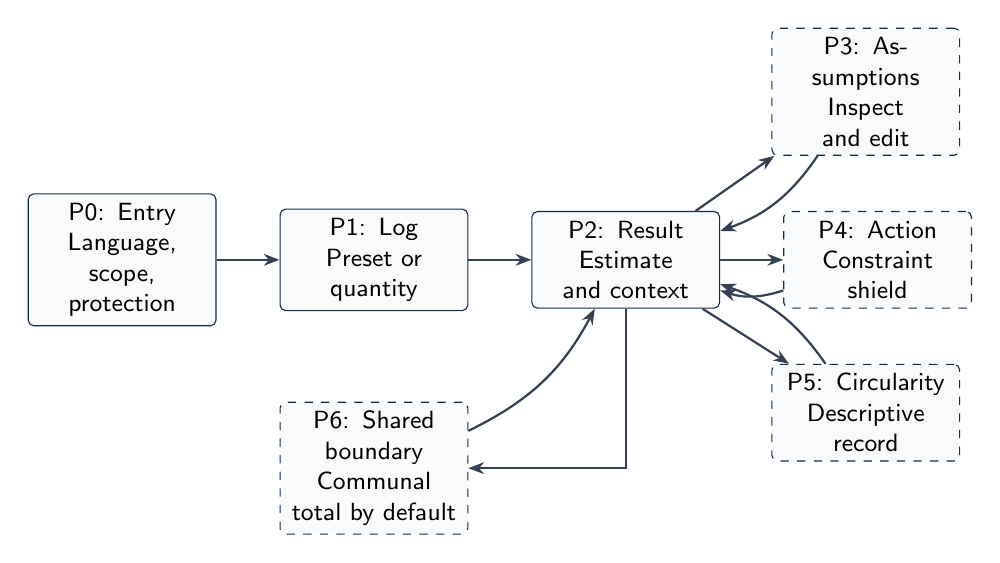
\begin{tikzpicture}[
  node distance=0.9cm and 0.8cm,
  state/.style={draw=AcademicNavy, rounded corners=2pt, fill=BgLight,
                text width=2.15cm, minimum height=0.9cm, align=center,
                font=\small},
  optional/.style={state, dashed},
  flow/.style={-{Stealth[length=2mm]}, thick, draw=AcademicSlate}
]
\node[state] (p0) {P0: Entry\\Language, scope, protection};
\node[state, right=of p0] (p1) {P1: Log\\Preset or quantity};
\node[state, right=of p1] (p2) {P2: Result\\Estimate and context};
\node[optional, above right=0.7cm and 0.65cm of p2] (p3) {P3: Assumptions\\Inspect and edit};
\node[optional, right=of p2] (p4) {P4: Action\\Constraint shield};
\node[optional, below right=0.7cm and 0.65cm of p2] (p5) {P5: Circularity\\Descriptive record};
\node[optional, below=1.15cm of p1] (p6) {P6: Shared boundary\\Communal total by default};
\draw[flow] (p0) -- (p1);
\draw[flow] (p1) -- (p2);
\draw[flow] (p2) -- (p3);
\draw[flow] (p2) -- (p4);
\draw[flow] (p2) -- (p5);
\draw[flow] (p2) |- (p6);
\draw[flow] (p3) to[bend left=18] (p2);
\draw[flow] (p4) to[bend left=18] (p2);
\draw[flow] (p5) to[bend right=18] (p2);
\draw[flow] (p6) to[bend right=18] (p2);
\end{tikzpicture}
\caption{Conceptual state-transition flow. Solid nodes show the core journey; dashed nodes represent optional branches. The diagram describes intended navigation, not implemented behaviour.}
\label{fig:state-flow}
\end{figure}

\newpage

% =========================================================================
% PROTOTYPE PAGE 1: MASTER ARCHITECTURAL FLOW (1 IMAGE)
% =========================================================================
\begin{figure}[H]
    \centering
    \renderpic{pic1.png}{0.98\textwidth}{0.78\textheight}
    \caption{Master Architectural Wireframe Grid (\texttt{pic1.png}) showing the complete offline state topology across States P0--P6.}
    \label{fig:master-wireframe}
\end{figure}

\newpage

% =========================================================================
% PROTOTYPE PAGE 2: STATES P0, P1, P2, P3 (EXACTLY 4 IMAGES)
% =========================================================================
\begin{figure}[H]
    \centering
    \begin{minipage}[t]{0.48\textwidth}
        \centering
        \renderpic{pic2.png}{\linewidth}{0.37\textheight}
        \vspace{2pt}
        {\footnotesize \textbf{(a) State P0 (\texttt{pic2.png}):} Entry, Language \& Scope.}
    \end{minipage}\hfill
    \begin{minipage}[t]{0.48\textwidth}
        \centering
        \renderpic{pic3.png}{\linewidth}{0.37\textheight}
        \vspace{2pt}
        {\footnotesize \textbf{(b) State P1 (\texttt{pic3.png}):} 2-Tap Presets \& Manual Logger.}
    \end{minipage}

    \vspace{0.6cm}

    \begin{minipage}[t]{0.48\textwidth}
        \centering
        \renderpic{pic4.png}{\linewidth}{0.37\textheight}
        \vspace{2pt}
        {\footnotesize \textbf{(c) State P2 (\texttt{pic4.png}):} Result \& What-If Simulator.}
    \end{minipage}\hfill
    \begin{minipage}[t]{0.48\textwidth}
        \centering
        \renderpic{pic5.png}{\linewidth}{0.37\textheight}
        \vspace{2pt}
        {\footnotesize \textbf{(d) State P3 (\texttt{pic5.png}):} Provenance \& Assumptions Audit.}
    \end{minipage}
    \caption{Low-fidelity wireframes for States P0, P1, P2, and P3 enforcing Epics E1, E2, E5, E6, and E9.}
    \label{fig:wireframes-p0-p3}
\end{figure}

\newpage

% =========================================================================
% PROTOTYPE PAGE 3: STATES P4, P5, P6 (EXACTLY 3 IMAGES)
% =========================================================================
\begin{figure}[H]
    \centering
    \begin{minipage}[t]{0.48\textwidth}
        \centering
        \renderpic{pic6.png}{\linewidth}{0.37\textheight}
        \vspace{2pt}
        {\footnotesize \textbf{(a) State P4 (\texttt{pic6.png}):} Constraint Shield \& Agency Options.}
    \end{minipage}\hfill
    \begin{minipage}[t]{0.48\textwidth}
        \centering
        \renderpic{pic7.png}{\linewidth}{0.37\textheight}
        \vspace{2pt}
        {\footnotesize \textbf{(b) State P5 (\texttt{pic7.png}):} Descriptive Circular Habit Record.}
    \end{minipage}

    \vspace{0.6cm}

    \begin{minipage}[t]{0.52\textwidth}
        \centering
        \renderpic{pic8.png}{\linewidth}{0.37\textheight}
        \vspace{2pt}
        {\footnotesize \textbf{(c) State P6 (\texttt{pic8.png}):} Shared Household Boundary \& Voluntary Opt-In.}
    \end{minipage}
    \caption{Low-fidelity wireframes for States P4, P5, and P6 enforcing Epics E3, E4, E7, E13, and E14.}
    \label{fig:wireframes-p4-p6}
\end{figure}

\clearpage

% =========================================================================
% SECTION 6: EVALUATION PLAN, PROJECT MANAGEMENT & AGILE REFLECTION
% =========================================================================

\subsection{Calculation Boundaries and Assumption Register}
D1 explicitly labels the scenario factors below as illustrative assumptions requiring verification. They are therefore presented as scenario inputs, not authoritative emission factors or measured local averages. In particular, the electricity example uses kg CO$_2$ (not kg CO$_2$e) because that is how D1 defines the scenario calculation. The broader footprint concept may use kg CO$_2$e where a defensible lifecycle factor is available; each activity therefore needs an explicit unit and system boundary.

\begin{table}[H]
\centering
\small
\begin{tabularx}{\textwidth}{@{}p{3.0cm}p{2.8cm}X@{}}
\toprule
\textbf{Parameter} & \textbf{D1 value} & \textbf{Required D2 treatment} \\
\midrule
Grid factor & 0.716 kg CO$_2$/kWh & Provisional illustrative assumption; show source/year as unverified until the team checks the cited CEA document. Do not label it kg CO$_2$e. \\
Electricity tariff & Rs. 8/kWh & Assumed tariff for arithmetic examples, not a universal Indian rate. Label Rs. 1,344 as estimated cost for 168 kWh, not savings. \\
Bus factor and trip distance & 0.015 kg CO$_2$/passenger-km; 15 km & Both are illustrative. A bus-trip comparison is conditional on these assumptions and must show them. \\
Water flow and bucket size & 7.5 L/min; 15 L & Water-volume comparison only; it is not a carbon equivalence. \\
AC power and WFH days & 1.5 kW; 14 days/month & Illustrative scenario assumptions. State them alongside the 21 kWh estimate. \\
\bottomrule
\end{tabularx}
\caption{Assumptions inherited from D1 and their disclosure requirements.}
\label{tab:assumptions}
\end{table}

\section{Formative Evaluation Plan and Agile Project Management}

\subsection{Formative Evaluation Plan (Testing RQ1--RQ3)}
To prepare for Deliverable 3, States P0--P6 are intended to support a formative think-aloud evaluation with a small convenience sample of COMP2300 participants. This is a proposed plan, not completed user testing. Avoid collecting sensitive personal data and report sample limitations.
\begin{itemize}
    \item \textbf{Task 1 --- Low-Friction Preset Logging (\textbf{RQ2}, States P0--P1):} Participants select \textit{Plain Hindi} or \textit{English} in State P0 and log a $168.0\text{ kWh}$ home electricity routine using a State P1 preset. \textit{Measures:} task completion rate, elapsed time, number of actions, input errors, and requests for assistance. \textit{Provisional success target:} at least 4 of 5 participants complete the familiar preset task without assistance in 60 seconds or less and with no more than two logging actions. This small sample is formative and cannot establish population-wide usability.
    \item \textbf{Task 2 --- Tangible Equivalent \& What-If Comprehension (\textbf{RQ1}, States P2--P3):} Participants explain what the displayed electricity result and Rupee estimate represent, identify the provisional factor and its unit, and interpret the optional AC comparison. \textit{Measures:} correct explain-back of the formula, distinction between cost and saving, recognition that water/currency are contextual comparators rather than carbon equivalents, and ability to locate the factor's source/year status. \textit{Provisional success target:} at least 4 of 5 participants correctly explain the calculation boundary and distinguish estimated cost from savings after using the interface.
    \item \textbf{Task 3 --- Constraint Shield, Circular Record \& Shared Boundary (\textbf{RQ3}, States P4--P6):} Participants identify the protected-routine state, record a phone repair descriptively, and inspect the communal-total and voluntary opt-in boundary. \textit{Measures:} correct identification of the protected state, whether users believe the tool is assigning blame, and whether they understand that another resident's individual share is not inferred. \textit{Provisional success target:} at least 4 of 5 participants correctly explain the protection and consent rules; any participant interpreting the interface as assigning blame or exposing another resident's usage triggers a design review.
\end{itemize}

For each task, the moderator records completion, time, observable errors, assistance, and a short post-task explain-back. A brief Single Ease Question (SEQ) may be used after each task, followed by an open-ended debrief on clarity, perceived pressure, and trust. These measures are intended to identify usability problems and refine the prototype; they are not a statistically powered validation study.

\subsection{Sprint 1 Plan, Risk Register, and Retrospective Reflection}
Table \ref{tab:risk-log} summarises our active project risk register and mitigation controls moving into Deliverable 3 and Sprint 1 (Deliverable 4).

\begin{table}[H]
\centering
\small
\renewcommand{\arraystretch}{1.35}
\begin{tabularx}{\textwidth}{@{} p{1.2cm} p{3.4cm} c X @{}}
\toprule
\rowcolor{AcademicNavy}
\textcolor{white}{\textbf{ID}} & \textcolor{white}{\textbf{Identified Risk}} & \textcolor{white}{\textbf{Severity}} & \textcolor{white}{\textbf{Mitigation \& Contingency Strategy}} \\
\midrule
\textbf{R1} & D1-to-D2 requirement drift across personas or epics. & High & Use the D1-to-D2 mapping in this report as the baseline and verify each epic/persona/scenario link during backlog refinement; record unresolved mappings as open traceability actions. \\
\rowcolor{RowAlt}
\textbf{R2} & Prototype fidelity penalty (looking too polished or coded in D2). & High & Keep the Figma artefacts at wireframe fidelity and use hand-drawn supplements only to clarify unresolved states; avoid implementation detail that makes the prototype appear to be a coded product. \\
\textbf{R3} & Uneven GitLab commit visibility or member unavailability in Sprint 1. & Medium & Plan implementation work across domain models and JSON persistence, FXML views, and ViewModels/tests; use branch and merge-request review to make ownership and integration visible during Sprint 1. \\
\bottomrule
\end{tabularx}
\caption{Deliverable 2 Risk Register and Mitigation Controls.}
\label{tab:risk-log}
\end{table}

\textbf{Product Reflection (Sprint Review):} Converging on Concept C resolved the core design tension uncovered in Deliverable 1: serving low-literacy or time-poor users (\textbf{P1, P4, P6}) alongside rigorous domain researchers (\textbf{P2}). Separating the 2-tap preset flow (States P0--P2) from the on-demand Provenance Inspector (State P3) achieved progressive disclosure without cluttering the primary interface.

\textbf{Process Reflection:} The D2 synchronisation pass highlighted the risk of losing persona-specific constraints when requirements are consolidated into broad user stories. The traceability review keeps the six D1 personas, four scenarios, and fourteen epics visible in the design register. For the next increment, the team will use milestone-tagged GitLab issues to assign implementation tasks and track verification evidence.

% =========================================================================
% SECTION 7: SYSTEM ARCHITECTURE AND TECHNICAL DESIGN BRIEF (PIC 9)
% =========================================================================
\section{System Architecture and Technical Design Brief}
As a proposed implementation direction for maintainability and the local-first privacy constraints defined in Epics \textbf{E5} and \textbf{E14}, the target Java 21 and JavaFX application could use a modular \textbf{Model-View-ViewModel (MVVM)} pattern coupled with the \textbf{Strategy Pattern} (Figure \ref{fig:proposed-architecture}):

\begin{itemize}
    \item \textbf{Presentation Layer (JavaFX \texttt{.fxml} Views):} Consists of passive UI views (\texttt{SimpleDashboardView}, \texttt{HouseholdHubView}, \texttt{AssumptionsAuditView}) that bind declaratively to ViewModel `ObservableProperties`. A future English/Plain Hindi resource bundle and optional comparison control can update the view reactively.
    \item \textbf{ViewModel Layer (State \& Boundary Enforcement):} Mediates UI state (\texttt{DashboardViewModel}, \texttt{HouseholdViewModel}, \texttt{AuditViewModel}) and enforces socio-technical rules—such as masking individual room attributions in State P6 unless the voluntary `isAttributionOptedIn()` property is explicitly set to `true`, and suppressing action nudges when the State P0 safety-lock flag is active.
    \item \textbf{Model \& Service Layer (Strategy Pattern --- Open/Closed Principle):} An `EmissionCalculationStrategy` interface abstracts domain logic across concrete implementations (`ApplianceWaterCalculator`, `TransportCalculator`, and `QuickCommerceCalculator`). These calculators read visible parameters ($0.716\text{ kg CO}_2\text{/kWh}$ (provisional illustrative assumption; verify source and year before treating as authoritative) grid factor, $\text{Rs. }8.00\text{/kWh}$ tariff) from `AssumptionsConfig` and pass results to `UnitEquivalencyConverter` to generate Rupee, bucket, and bus-trip equivalents.
    \item \textbf{Data Persistence Layer (100\% Offline Local Storage):} `LocalRepository` serialises user logs and custom assumption configurations into local JSON files via Jackson/Gson. Local CSV export is deferred to the E9 Should-Have increment; the core logging flow does not require external network calls.
\end{itemize}


\begin{figure}[H]
\centering
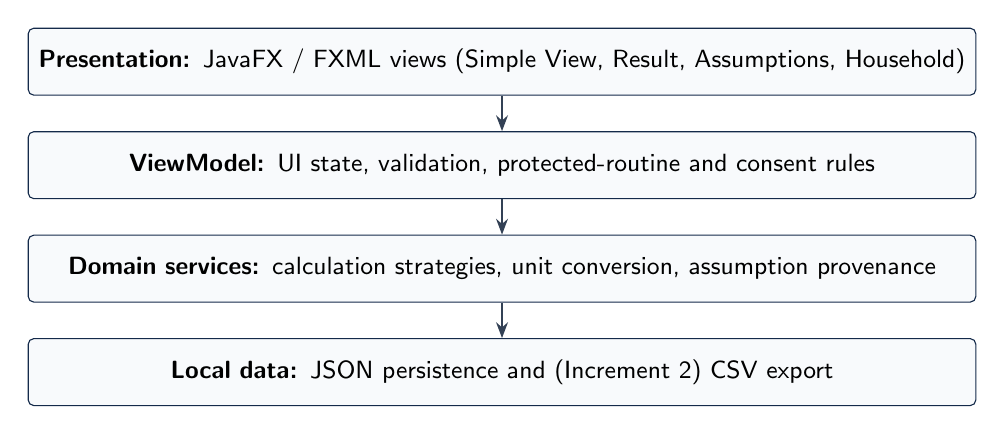
\begin{tikzpicture}[
  layer/.style={draw=AcademicNavy, rounded corners=2pt, fill=BgLight,
                text width=11.8cm, minimum height=0.85cm, align=center,
                font=\small},
  arrow/.style={-{Stealth[length=2mm]}, thick, draw=AcademicSlate}
]
\node[layer] (view) {\textbf{Presentation:} JavaFX / FXML views (Simple View, Result, Assumptions, Household)};
\node[layer, below=0.45cm of view] (vm) {\textbf{ViewModel:} UI state, validation, protected-routine and consent rules};
\node[layer, below=0.45cm of vm] (service) {\textbf{Domain services:} calculation strategies, unit conversion, assumption provenance};
\node[layer, below=0.45cm of service] (repo) {\textbf{Local data:} JSON persistence and (Increment 2) CSV export};
\draw[arrow] (view) -- (vm);
\draw[arrow] (vm) -- (service);
\draw[arrow] (service) -- (repo);
\end{tikzpicture}
\caption{Proposed layered architecture for later JavaFX implementation. It is a design proposal, not evidence of implemented classes or tested code.}
\label{fig:proposed-architecture}
\end{figure}




% =========================================================================
% REFERENCES
% =========================================================================
\begin{thebibliography}{9}
\bibitem{hoffmann2024} S. Hoffmann, W. Lasarov, H. Reimers and M. Trabandt. 2024. Carbon footprint tracking apps: What drives user engagement and behavioral change? \emph{Journal of Cleaner Production} 434, 139981. DOI: \href{https://doi.org/10.1016/j.jclepro.2023.139981}{10.1016/j.jclepro.2023.139981}.
\bibitem{lasarov2024} W. Lasarov, S. Hoffmann, R. Mai and J. Schleich. 2024. Carbon footprint tracking apps: the spillover effects of feedback and goal-activating appeals. \emph{Ecological Economics} 226, 108354. DOI: \href{https://doi.org/10.1016/j.ecoleco.2024.108354}{10.1016/j.ecoleco.2024.108354}.
\bibitem{brynjarsdottir2012} H. Brynjarsdottir, M. Hakansson, J. Pierce, E. Baumer, C. DiSalvo and P. Sengers. 2012. Sustainably unpersuaded: How persuasion narrows our vision of sustainability. In \emph{Proc. ACM CHI '12}. ACM, 947--956. DOI: \href{https://doi.org/10.1145/2207676.2208539}{10.1145/2207676.2208539}.
\bibitem{lee2021} J. Lee, O. Taherzadeh and K. Kanemoto. 2021. The scale and drivers of carbon footprints in households, cities and regions across India. \emph{Global Environmental Change} 66, 102205. DOI: \href{https://doi.org/10.1016/j.gloenvcha.2020.102205}{10.1016/j.gloenvcha.2020.102205}.
\bibitem{mohanty2023} V. Mohanty, A. Filipowicz, N. Bravo, S. Carter and D. A. Shamma. 2023. Save a tree or 6 kg of CO2? In \emph{Proc. ACM CHI '23}. ACM. DOI: \href{https://doi.org/10.1145/3544548.3580675}{10.1145/3544548.3580675}.
\bibitem{shi2021} S. Shi and J. Yin. 2021. Global research on carbon footprint: A scientometric review. \emph{Environmental Impact Assessment Review} 89, 106571. DOI: \href{https://doi.org/10.1016/j.eiar.2021.106571}{10.1016/j.eiar.2021.106571}.
\end{thebibliography}

\end{document}